\section{Three Dimensional Analysis}
\noindent This section extends the analysis of the two dimensional approach, and is intended to explore and analyse the  three dimensional flow features. It was surmised that three dimensional flow allows for more complex flow behaviour, that may significantly affect an undertray's overall performance. This part of the report will be divided into 3D open flow, and undertray prototype with bluff body analyses.

\subsection{3D Open Flow}
This analysis is an extension to three dimensions of the 2D open flow cases. The purpose of this analysis to investigate further the flow features that develop in an undertray in a three dimensional manner, which might plausibly affect its performance.

\subsubsection{Geometry and Mesh Generation}
An identical 2D sketch from geometry 3 of the 2D open flow section was used, which then extruded to a car-realistic 1 meter thickness. A skirt was added to both sides of the rear diffuser. These skirts were used to improve flow isolation and to generate corner vortices, which help to improve flow attachment within the diffuser region. Fences were also added to later analyses to investigate the effects of vortex generators with respect to the generation of downforce. A sketch of the geometry can be seen in Figure~\ref{fig:3D_OF_GEOM} below. 

\begin{figure}[!h]
    \centering
    \noindent\makebox[\textwidth]{
    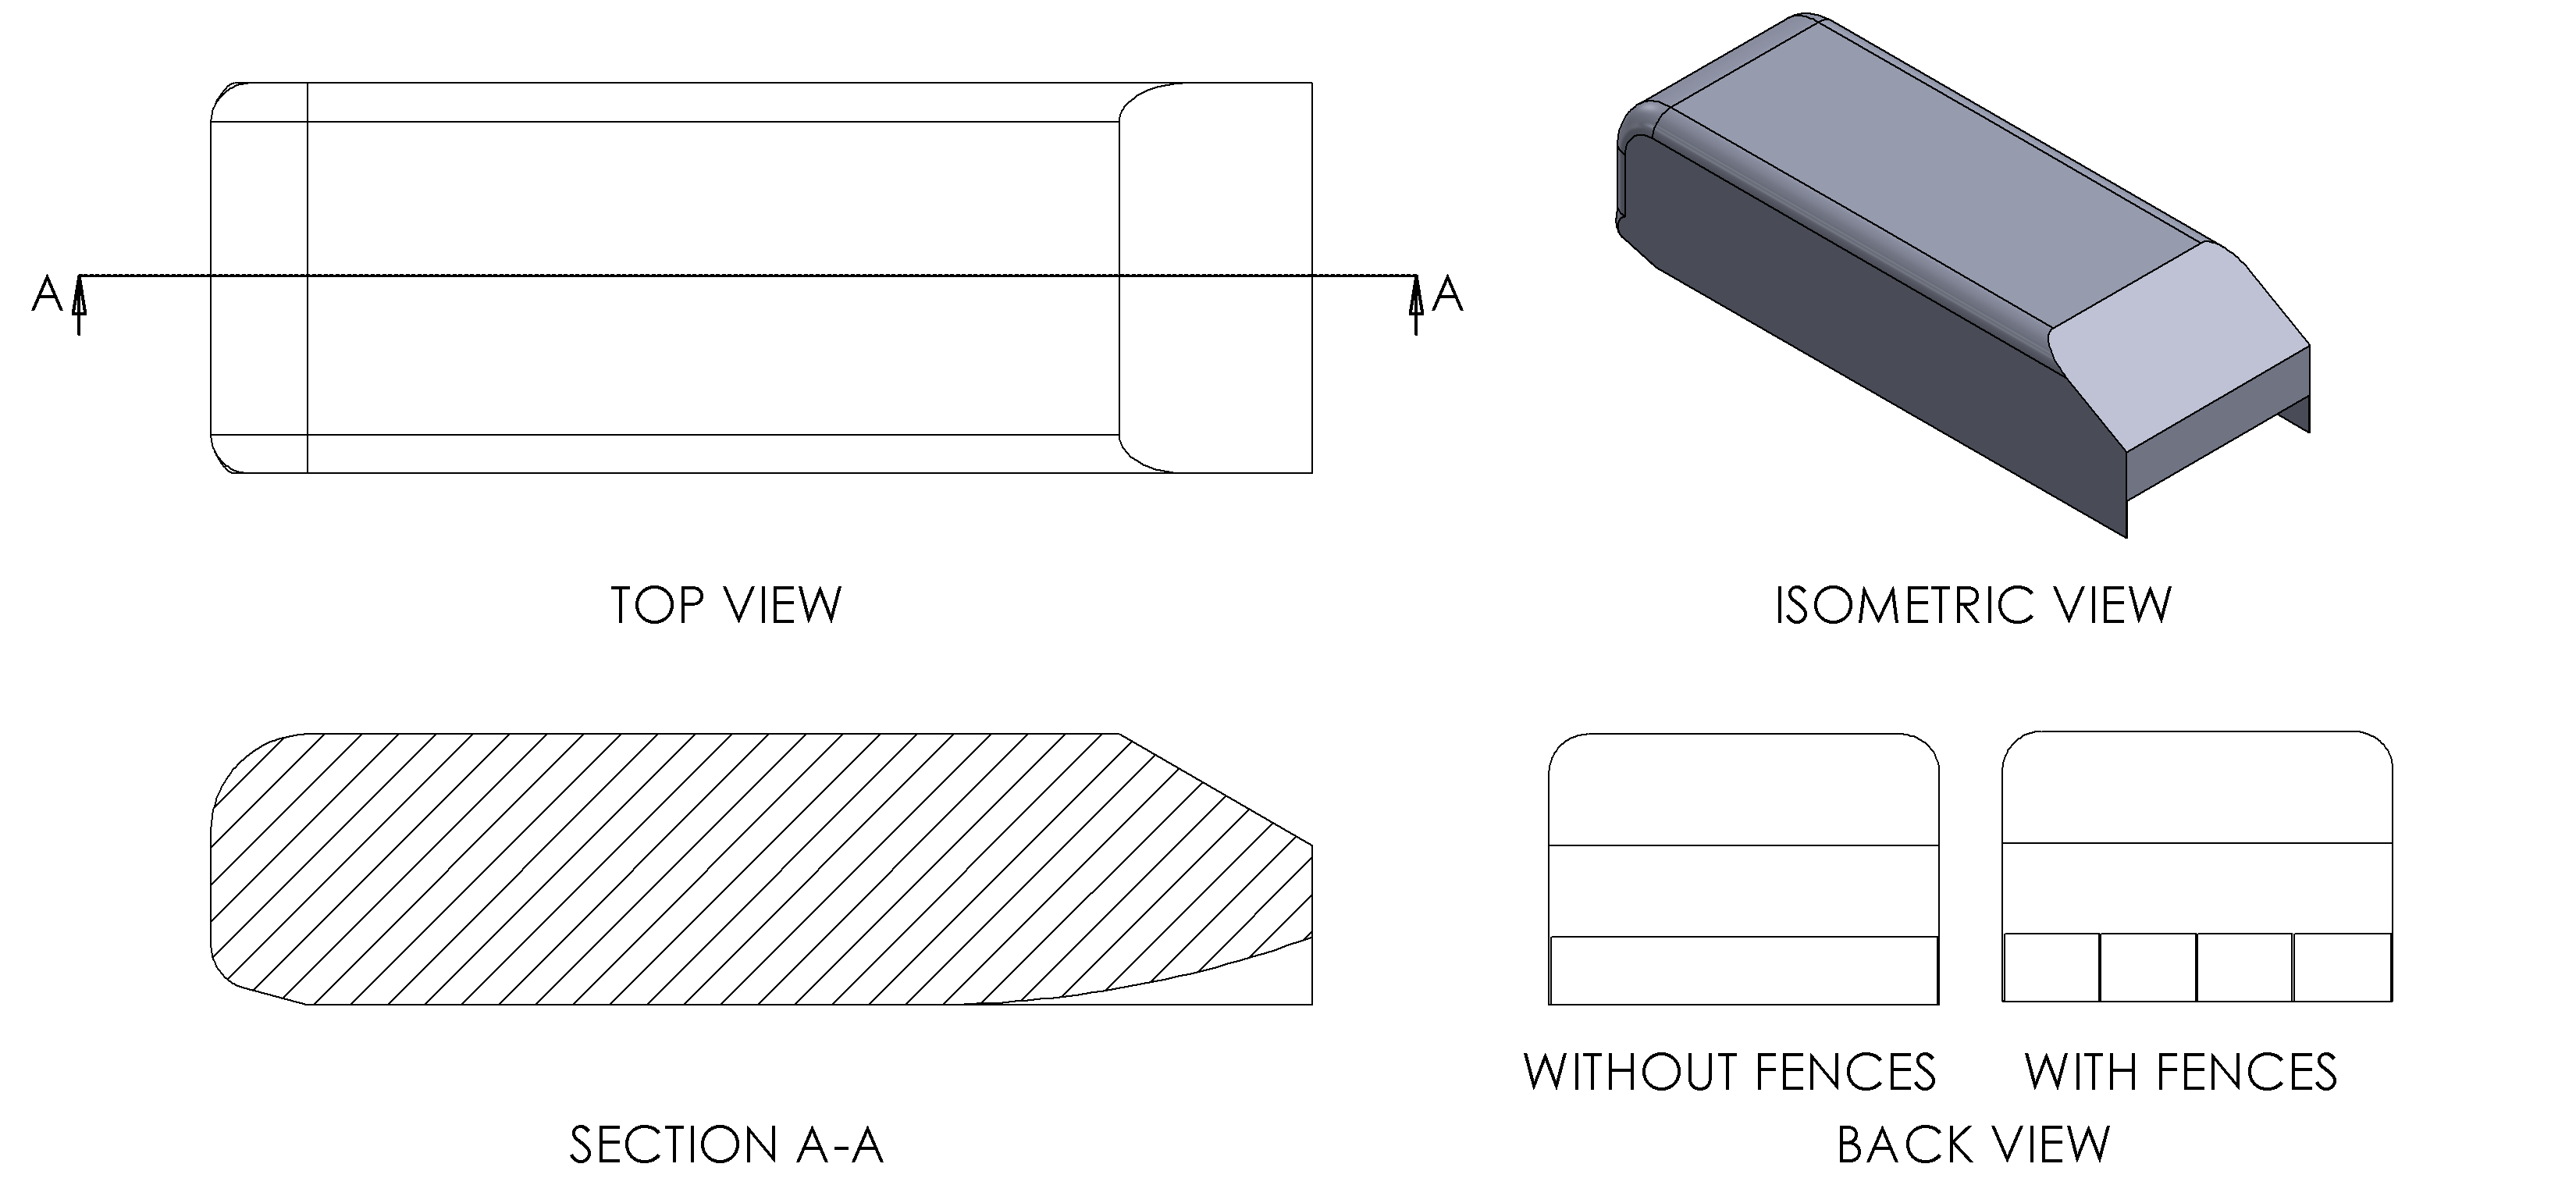
\includegraphics[width=0.8\textwidth]{Figures/3D_OF/3D_OF_D.PNG}}
    \caption{Geometry Generated for 3D Open-Flow Analysis.}
    \label{fig:3D_OF_GEOM}
\end{figure}

\noindent The CAD geometry was then imported into DesignModeler, where the fluid domain and body of influence were built.

The fluid domain was made with roughly 2 cars length forward, 5 behind, 3 top, and 3 side wise with 0.03 meters of ground clearance from the undertray's lowest point. Due to the symmetry of the body, a half model was used for the fluid domain to minimise the mesh element count. A body of influence (BOI), with dimensions of  $6 \times 1 \times 7$ meters was created using a box feature around the body to increase the mesh density and capture the surrounding flow features.  % NON DIMENSIONALISED IT HOW MANY CAR LENGTH

\noindent A hybrid mesh was used, which is comprised of tetrahedrons and triangular prisms. Twenty inflation layers of triangular prism were applied near the wall to give a $y^+=1$. A max element size of 0.8 meters and 0.02 meters in the BOI generated a mesh with 1.3 to 1.5 elements for this analysis. This section's mesh quality is considered acceptable, with an average skewness of 1.9 and an aspect ratio of 80-90; however, a significant jump in size in the cells between the inflation layer and far-field fluid domain is considered not ideal. Detailed illustration of the fluid domain and the mesh can be seen in Figure~\ref{fig:3D_OF_MESH} Appendix C.

\subsubsection{Results and Discussions}
Due to the nature of the mesh, the $k-\omega$ SST model was used throughout this analysis to take advantage of the features of this particular transport model \cite{Ansys2006ModelingFlows}. The analyses will be grouped into four sets of geometries: varying diffuser angle with no inlet angle, varying diffuser angles with an inlet angle of 10 degrees, varying inlet angle with 10 degrees diffuser angle, and variable diffuser angle with three fences applied. Figure~\ref{fig:3D_OF_PLOT_COMPARE_ALL} below shows the comparison of lift and drag between all the variables.

\begin{figure}[htb!]
    \centering
    \noindent\makebox[\textwidth]{
    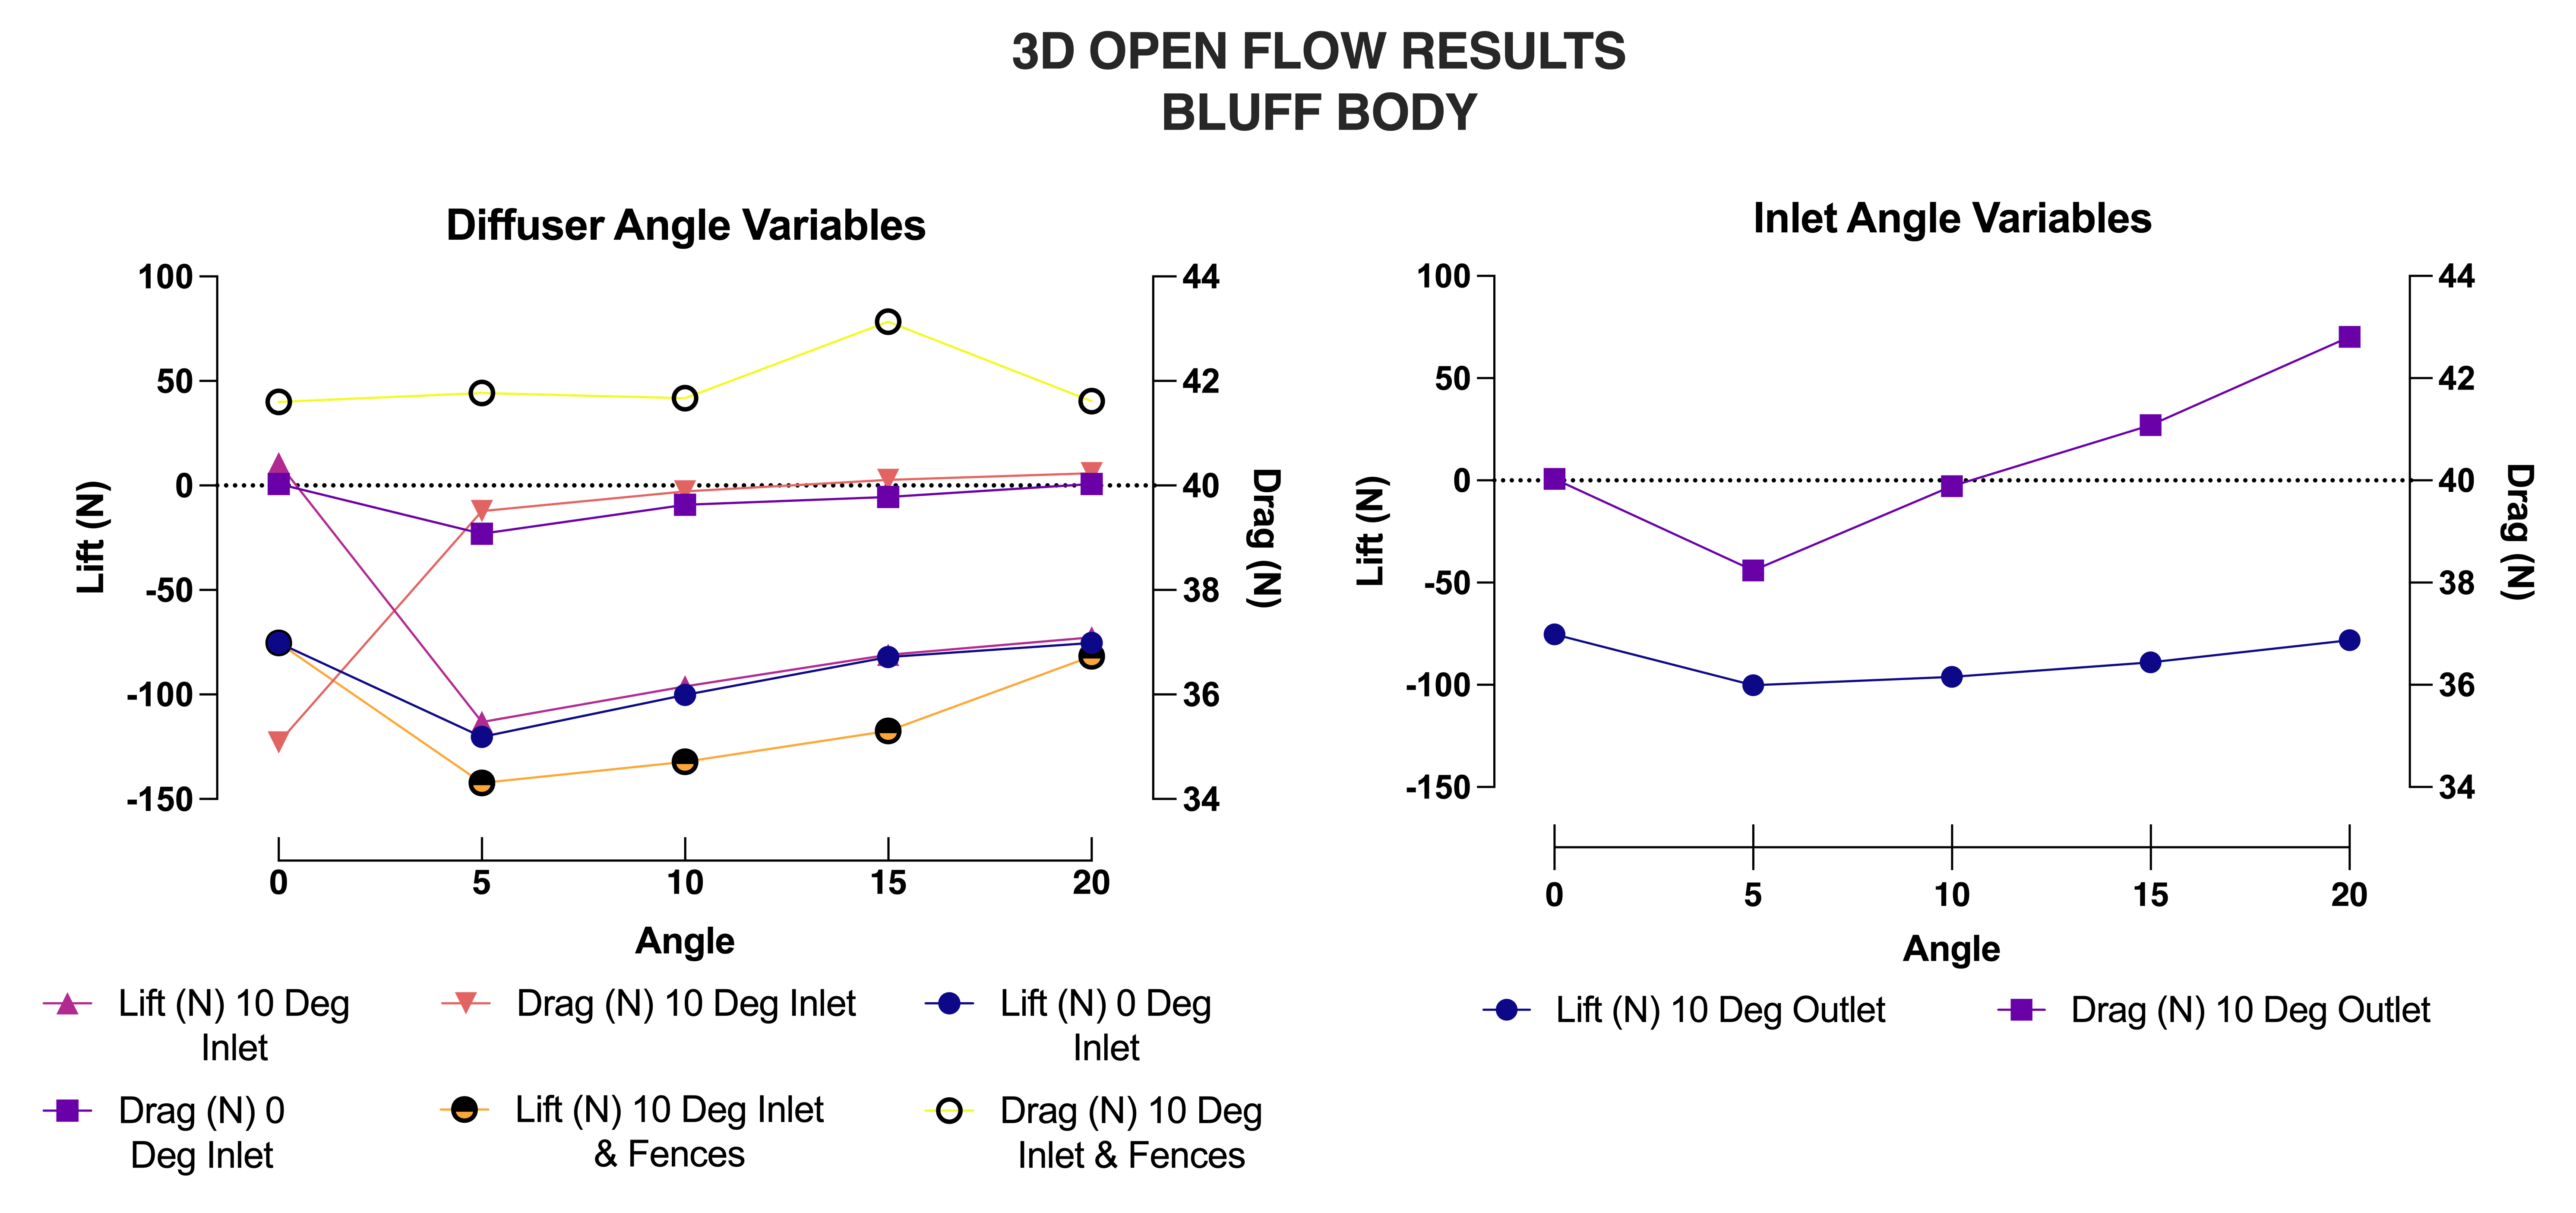
\includegraphics[width=0.9\textwidth]{Figures/Graph/3D_OF.png}}
    \caption{Lift and Drag Variation of Diffuser (left) and Inlet (right) Angle for All Geometry Configurations.}
    \label{fig:3D_OF_PLOT_COMPARE_ALL}
\end{figure}

\noindent The values of lift and drag as computed represent the values for the half body. Once more, a similar trend emerged as with the 2D open flow geometry 3. The trend shows an increase in downforce at a 5 degrees diffuser angle, followed by the downforce falling linearly up to 20 degrees. In comparison with 2D open flow analysis, the average downforce of this analysis is significantly lower. This is due to the nature of the analysis which allows the accelerated flow in the undertray to be affected by the flow surrounding the body. This is in contrast to the 2D open-flow, in which the flow past the undertray is constrained to move solely in plane. 

In three dimensions, the lower pressure region in the undertray sucks in the air from the side of the car. The flow which entertained from the side consequently generates instability and separation on the underbody's accelerated flow \cite{Bouferrouk2014OnVehicles}. This phenomenon may reduce the effectiveness of the flow acceleration underneath, resulting in a lower downforce. This occurrence is illustrated in Figure~\ref{fig:Vector_suction_diagram} below, with the influence of the corner vortices occurring from the fore of the bluff body. 

\begin{figure}[!htb]
    \centering
    \noindent\makebox[\textwidth]{
    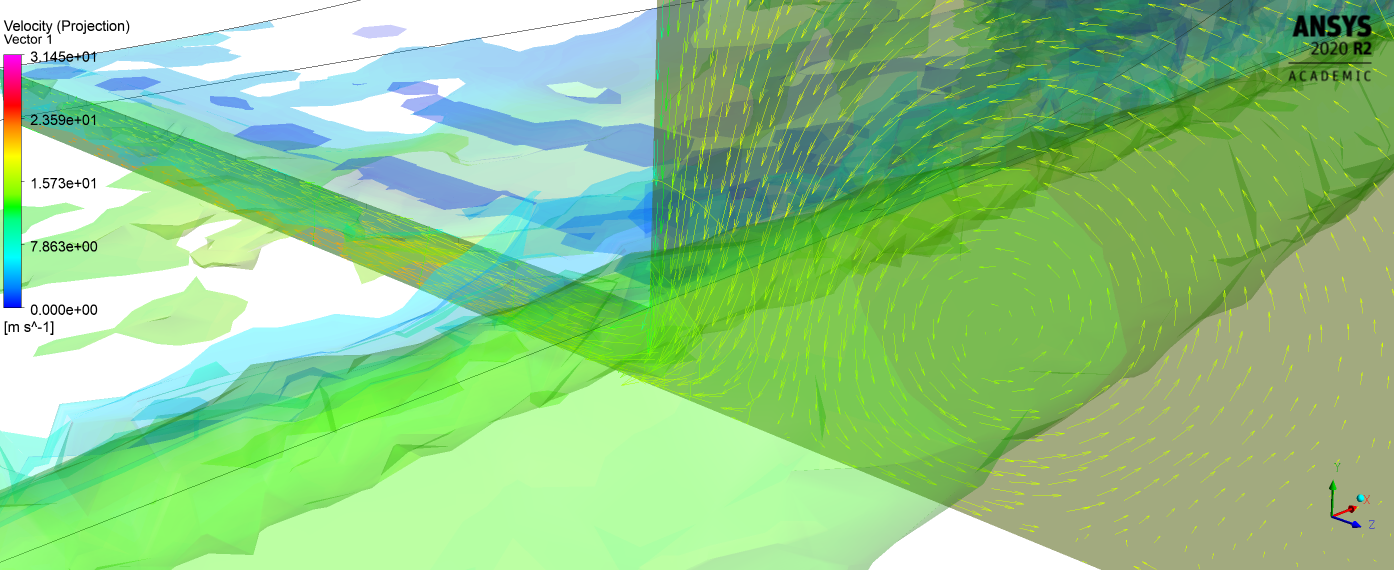
\includegraphics[width=0.8\textwidth]{Figures/3D_OF/3D_OF_VECTOR_SUCTION.png}}
    \caption{Vector Diagram of Velocity Flow on the Undertray's Cross-Section Indicating Flow Suction From The Side of The Body.}
    \label{fig:Vector_suction_diagram}
\end{figure}

\noindent The inlet angle elevation was simulated with 10 degrees diffuser angle. It can be examined that the effect of inlet angle elevation shows significant difference to the 2 dimensional analyses. Lift and drag of the bluff body reach its minimum at 5 degrees which then followed by lift and drag rise up to 20 degrees. As discussed in earlier section, stagnation point in the forepart of bluff body in 2 dimensional simulation creates separation point of flow direction to the top and bottom. However, in 3 dimensional case, the stagnation point separates the flow without consistent direction which create more complex flow features in the inlet region. An identical front cross-section of the car was made on the fore-flow of the body which became the initial location of streamline. \textbf{Figure \ref{fig:3D_OF_INLET_COMPARE} left} shows the streamline separation from the free flow to the surrounding body. Moreover, some of the streamline flow are leaked to the side, creating a trailing corner vortex \textbf{(middle)} hence reducing the intake acceleration in the undertray.  Compared to the 2 dimensional analysis, the flow that goes to the undertray stays without leaking or generate trailing vortex, which make the flow intake better, hence higher downforce. This explains the downforce degradation after 5 degrees, as the inlet angle increases, more airflow are leaking on the inlet region and creating bigger trailing vortex. Increase in drag comes from the skin friction as the flow is imposed by larger area with elevation of angle, and the trailing vortex which plausibly affect the flow on the throat (as discussed previously). It is worth noting that the changes of drag with inlet angle elevation is not significant and can be ignored, hence it was not used in  bluff body geometry with fences.

\begin{figure}[!htb]
    \centering
    \noindent\makebox[\textwidth]{
    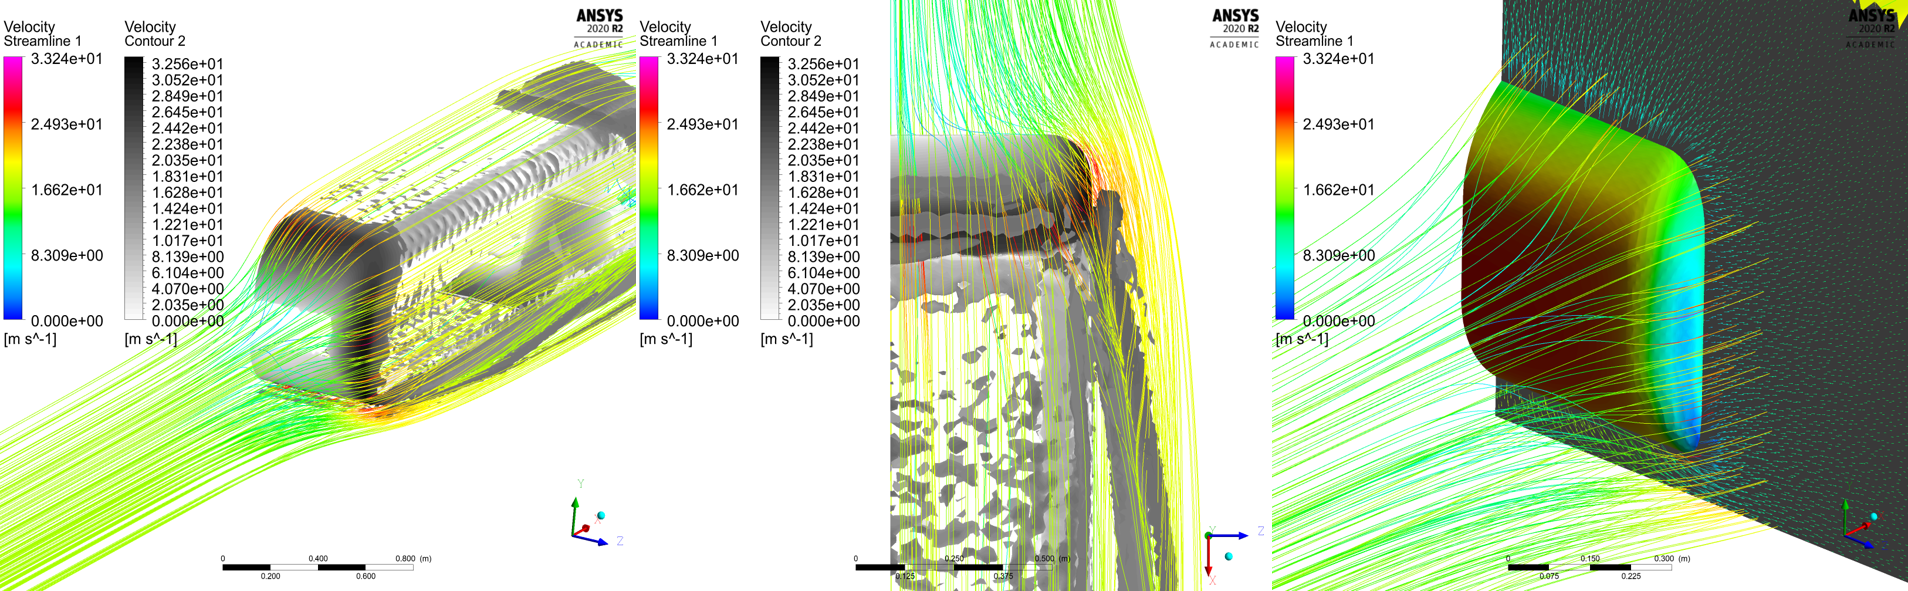
\includegraphics[width=1\textwidth]{Figures/3D_OF/3D_OF_INLET_COMPARE.png}}
    \caption{Fore-Flow Streamline Imposing The Bluff-Body and Occurrence of Leaking Indicated by The Trailing Vortex ($Q$-Criterion Isosurface) at The Inlet Region (left and middle), and Velocity Vector of The Flow Indicating Flow Leaks at The Inlet Region (right).} 
    \label{fig:3D_OF_INLET_COMPARE}
\end{figure}

\noindent Comparing the lift and drag with the diffuser varying with or without an inlet angle, the graphs exhibit an identical results except at 0 degrees. Here, there is a noticeable drop in downforce and drag, which is plausibly due to the diffuser's absence. A well-designed diffuser is important because it slowly expands the flow and allows the jet to stay attached to the undertray surface. Moreover, the side skirts in the diffuser allows the generation of corner vortices that help the flow to remain attached still further, hence increasing the overall downforce. ANSYS Post CFD allows the visualisation of $Q$-Criterion isosurfaces, which marks a vortex region ($Q > 0$) as where the anti-symmetric component of velocity gradient tensor is more dominating than the symmetric \cite{Holmen2012MethodsIdentification}. The corner vortex allows the boundary layer to stick on to the wall, slowing the pressure expansion hence the reduction in lift and drag. This phenomenon can be seen on Figure~\ref{fig:3D_OF_COMPARE_FENCES_SHEAR}, where the region in which the vortex is present has a higher wall shear stress than its surroundings, indicating flow attachment in the respective direction.

\begin{figure}[!htb]
    \centering
    \noindent\makebox[\textwidth]{
    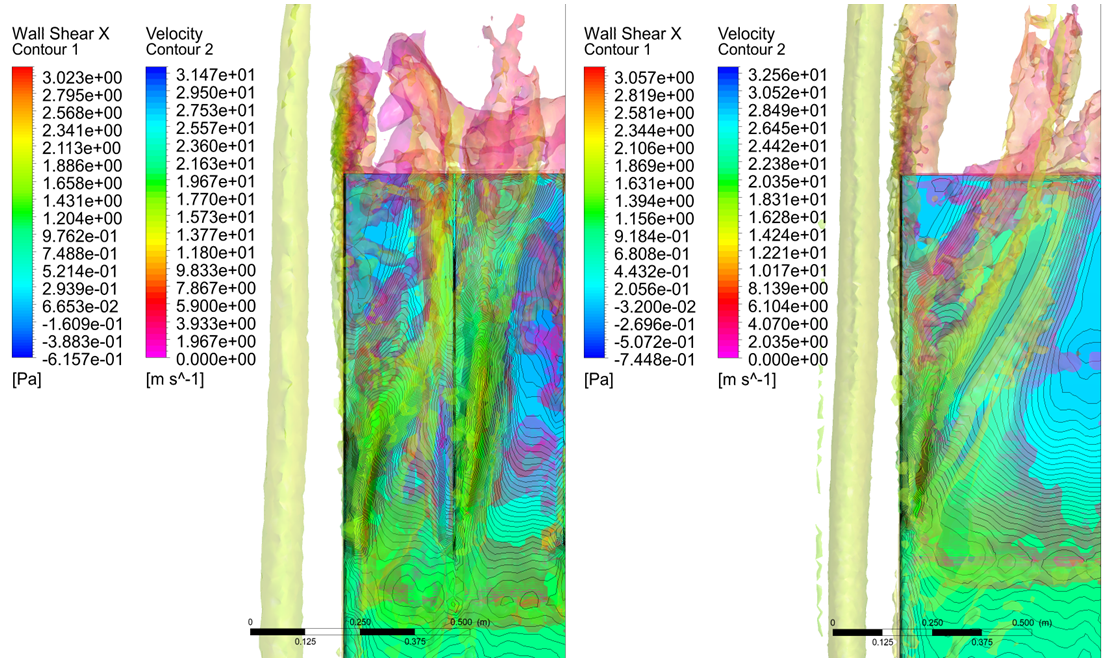
\includegraphics[width=0.65\textwidth]{Figures/3D_OF/3D_OF_COMPARE_FENCES.png}}
    \caption{Comparison of X Wall-Shear and Vortex Velocity ($Q$-Criterion Isosurface) Generated on The Diffuser Region With (left) and Without (right) Fences Applied.}
      \label{fig:3D_OF_COMPARE_FENCES_SHEAR}
\end{figure}

\noindent The next analysis incorporates fences (vertical partitions on the diffuser) to generate corner vortices to investigate their effects on the undertray's performance. The lift and drag plots shown in Figure~\ref{fig:3D_OF_PLOT_COMPARE_ALL} demonstrate an overall higher downforce compared to the bluff body without the fences. A similar concept of vortex generation applies. With the fences installed, there are more vortices generated along the diffuser. This reduces the flow separation in the x direction (flow direction), and maintains flow attachment, thus increasing the downforce. Figure~\ref{fig:3D_OF_COMPARE_FENCES_SHEAR} illustrates the presence of the extra vortices generated inside the diffuser by additional fences, and the smaller flow separation region indicated by non zero x-wall shear region. 

%TALK ABOUT SYMMETRY LIMITATION

\subsection{3D Undertray}
Overall previous analyses have given a fundamental understanding of flow behaviour, features, and performance trends of an underbody flow. This section of the report will utilise previous simulations to design several undertray prototypes that will be simulated using traced bluff-body of QFR car to achieve a realistic picture of the flow in real-life circumstances. The results documented then analysed thoroughly.

\subsubsection{Geometry and Mesh Generation}
\noindent Previous results have developed the knowledge of the trends in flow behaviour for the undertray's inlet and diffuser angles. Eight prototype designs were made based on interpreting these results and some engineering judgement from prior results. Several configurations were used to achieve the best results in the designs, including side diffuser, flat side-plate; dual variable diffuser; Gurney flaps; and variable vortex generators. These variables were all aimed at achieving the maximum performance of the undertray. All eight undertray prototype geometries can be seen in Figure~\ref{fig:UTP_D} in Appendix D.


%Explain the undertray geometry

\noindent An earlier project by McClune \cite{McClune2018DesignCar} analysed several undertray designs. However, the simulations undertaken consisted solely of the undertray; hence, unrealistic velocity and pressure fields were developed upon the top of the undertray. To overcome this issue, A bluff-body traced from the actual car was developed and installed to approximate the real QFR 2021 car's flow. Nonetheless, several simplifications were made for ease and computational performance, such as the suspension and tyres, which may disturb or pre-sculpt the oncoming flow before it enters the side undertray. Figure~\ref{fig:3D_UT_BB_SIMPLIFICATION} shows the QFR car simplification into a bluff body that fits above the undertray design.

\begin{figure}[!htb] 
    \centering
    \noindent\makebox[\textwidth]{
    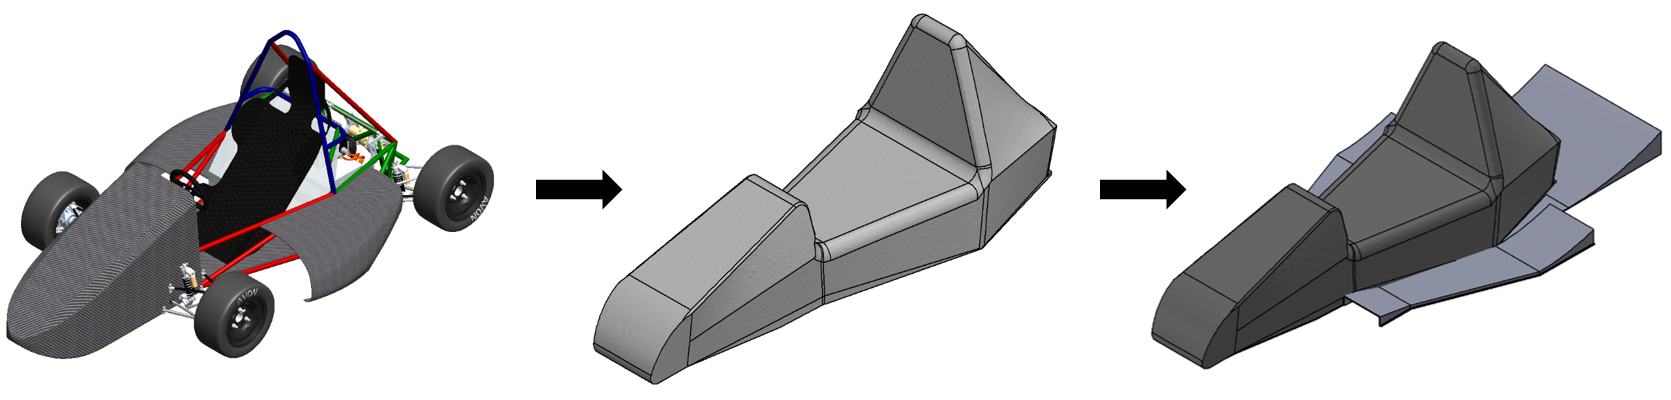
\includegraphics[width=0.8\textwidth]{Figures/UTP_FIGS/UT_BB_SIMPLIFY.png}}
    \caption{Simplification of QFR Car as an Undertray's Bluff Body to Simulate Realistic Flow Around The Body.}
      \label{fig:3D_UT_BB_SIMPLIFICATION}
\end{figure}

 \noindent Fluid-flow then generated using Design Modeller.  A partial model enclosed fluid-flow region was made with roughly 3 cars length behind, 1 forward, 1 top, and 1 side-way with 0.03 meters gap clearance from the lowest point of the undertray. To capture the flow feature in the undertray and bluff-body region, two Body of Influence (BOI) were incorporated. A bigger BOI with dimensions of 5 $\times$ 1.2 $\times$ 1.2 meters was generated to capture the flow surrounding the bluff body and an additional smaller BOI on the undertray region used 3 $\times$ 0.25 $\times$ 0.7 meters of dimension. The enclosed fluid flow generated can be seen on \textbf{figure \ref{fig:UTP_Fluid_flow} in Appendix D}
 
 \begin{figure}[!htb] 
    \centering
    \noindent\makebox[\textwidth]{
    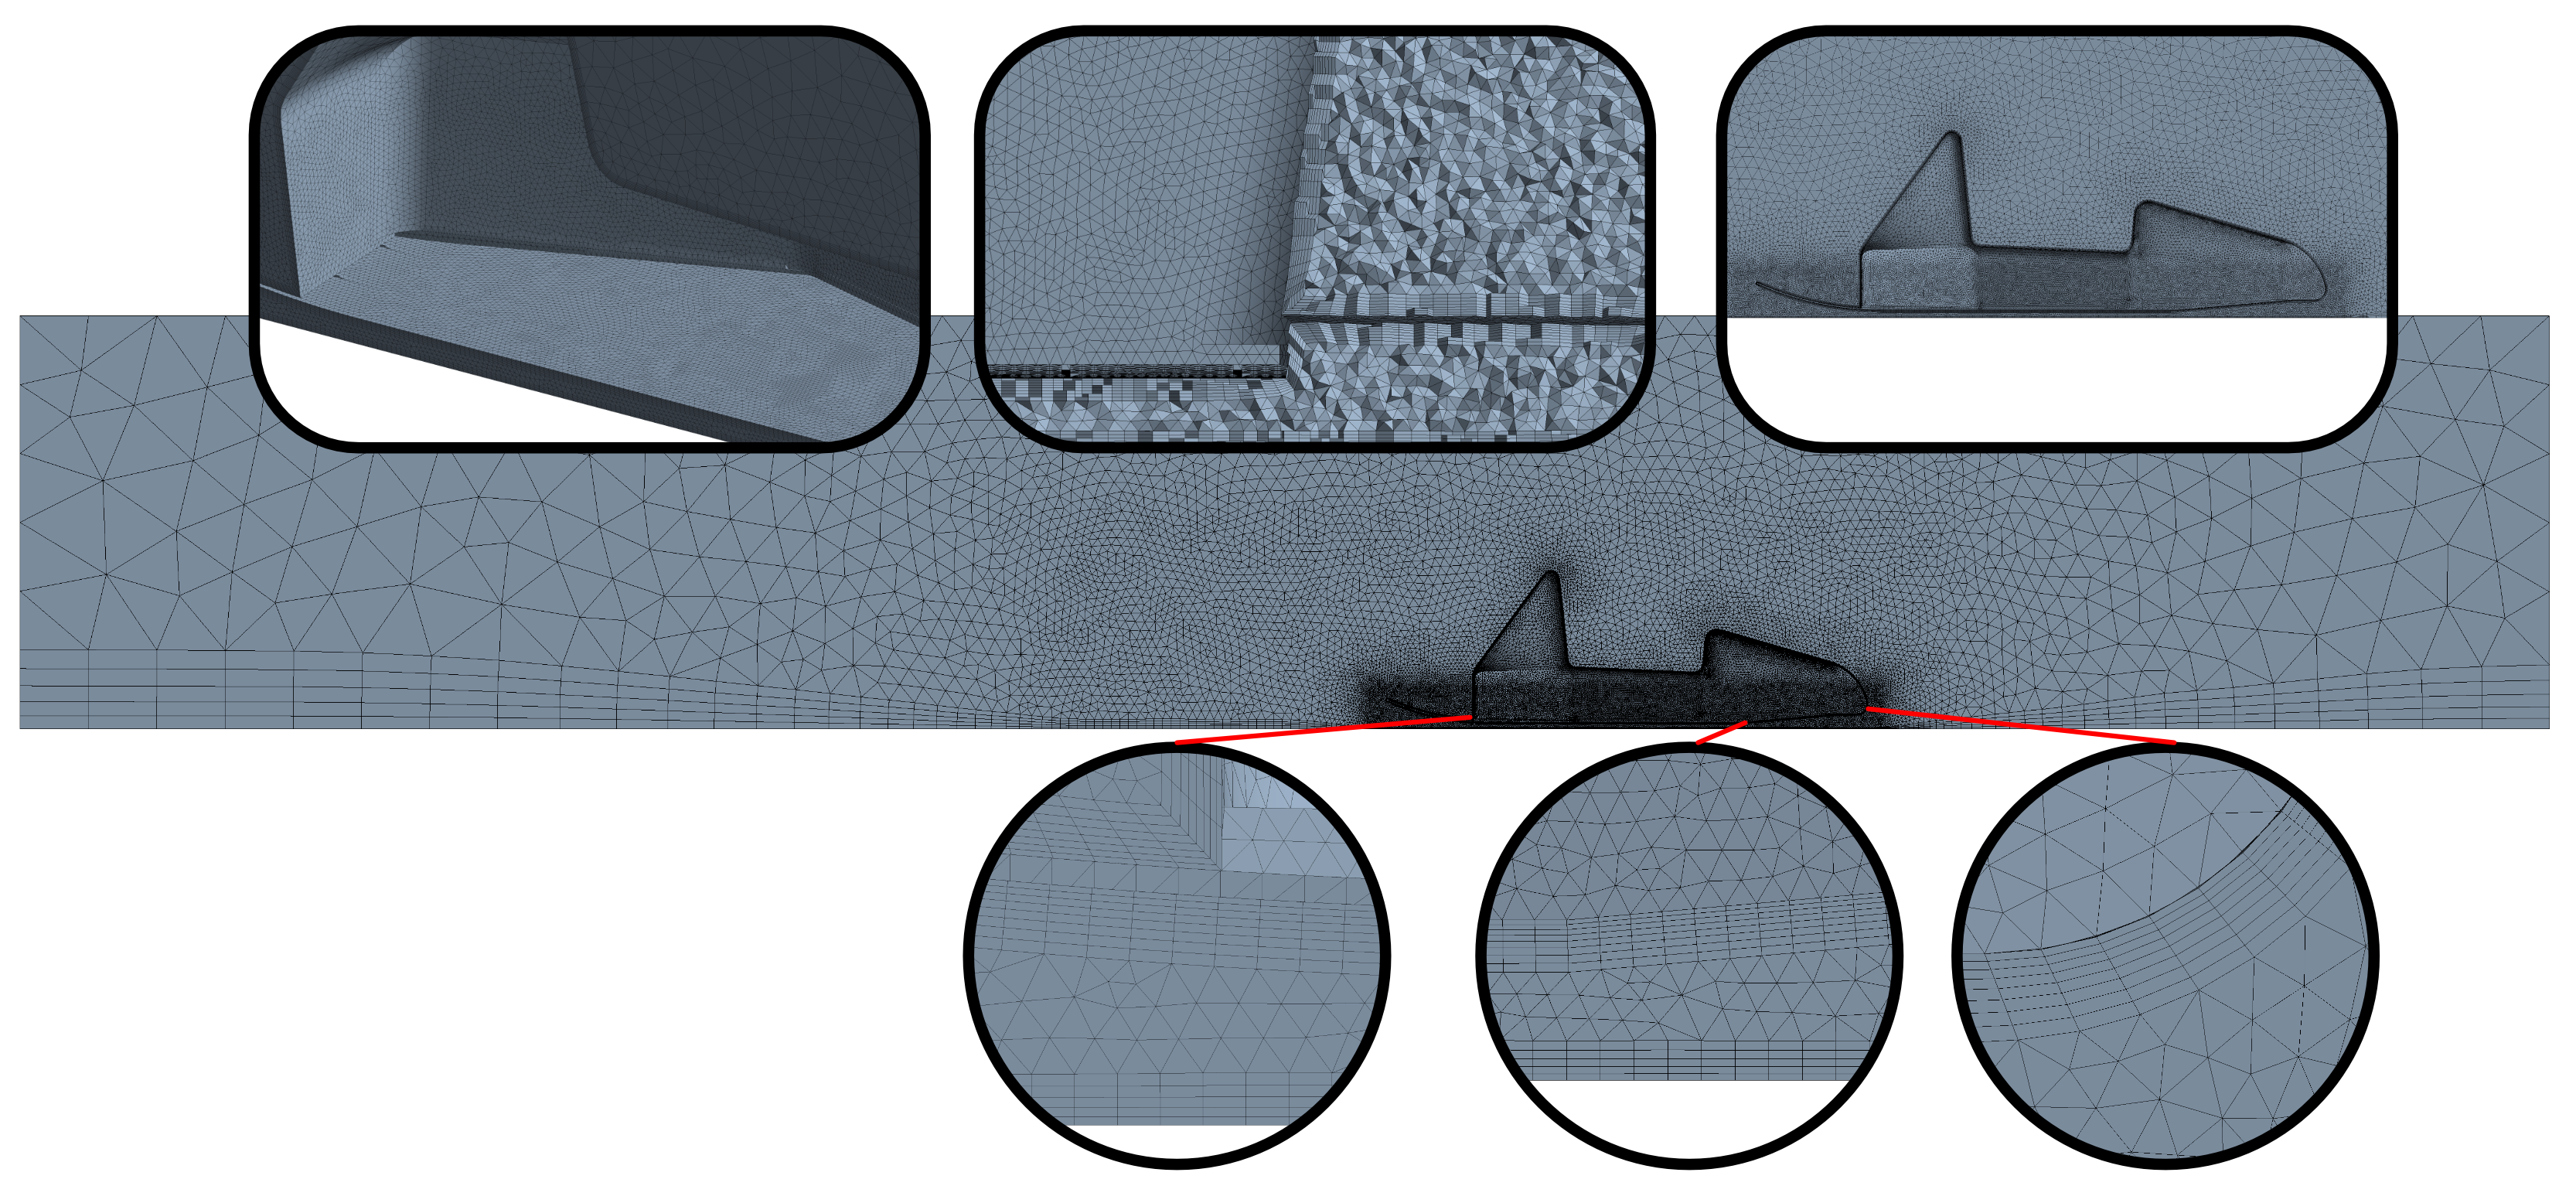
\includegraphics[width=0.9\textwidth]{Figures/UTP_FIGS/3D_UT_BB_MESH_COMPILE.png}}
    \caption{3D Hybrid Mesh Generated for Undertray Prototype Design With Bluff Body.}
    \label{fig:3D_UT_MESH}
\end{figure}

\noindent A hybrid mesh for 3D Undertray Prototype design is shown in figure \ref{fig:3D_UT_MESH} above. To capture details on the undertray region, 2 BOI were used on both car's surroundings and the undertray area. The first BOI used 0.05 meters of sizing and 0.008 for the second BOI near the undertray region with a cell growth rate of 1.1. Similarly to other analyses, inflation layers were used on the moving-floor and bluff body. $y^+$ = 1 was used near the body, with configurations of 8 inflation layer, first cell height of 0.00115 meters, and 1.1 cell growth rate. However, to reduce the jump cell size on the far-field and still capture the boundary layer in the undertray region, a smooth transition inflation layer was used on the floor region. Smooth transition of 0.272 (default) with five inflation later and 1.1 cell growth rate was used. As results, around 9.5 to 9.8 millions elements were generated with average element quality of 0.785, skewness of 0.206, and aspect ratio of 2.399, which put the overall quality of the mesh in a very good region \cite{Ansys2006ModelingFlows}.   

\subsubsection{Results and Discussion}
\textbf{Table \ref{UTB_RESULTS}} below shows the table of eight undertray simulation results to compare with similar simulation environment and settings. The bluff body alone was also simulated to be the base compared to the one with the undertray attached. It is worth noting that UTP stands for Undertray Prototype as a simplification in file and simulations naming convention.


\begin{table}[!htb]
\centering
\caption{Simulation Results of Undertray Prototype Designs.}\label{UTB_RESULTS}
\begin{tabularx}{0.95\textwidth}{ 
  | >{\centering\arraybackslash}X 
  | >{\centering\arraybackslash}X
  | >{\centering\arraybackslash}X
  | >{\centering\arraybackslash}X
  | >{\centering\arraybackslash}X
  | >{\centering\arraybackslash}X |
  }
\hline
\multirow{2}{*}{Design Name} & \multicolumn{2}{>{\hsize=\dimexpr2\hsize+2\tabcolsep+\arrayrulewidth\relax\centering}X|}{Full Body Results}  & \multirow{2}{*}{L/D Ratio} & \multicolumn{2}{>{\hsize=\dimexpr2\hsize+2\tabcolsep+\arrayrulewidth\relax\centering}X|}{Aerodynamics Improvement} \\ \cline{2-3} \cline{5-6}
 & Lift (N) & Drag (N) & & Lift (N) & Drag (N) \\
\hline

Bluff Body (Baseline)& -38.48 & 78.72 & -0.49 & 0 & 0\\
\hline
UTP0 & -106.26 & 59.81 & -1.78 & -67.79 & -18.91\\
\hline
UTP1 & -124.00 & 80.78 & -1.53 & -85.50 & 2.06\\
\hline
UTP2 & -222.59 & 68.23 & -3.26 & -184.12 & -10.49\\
\hline
UTP3 & -108.40 & 67.15 & -1.61 & -69.92 & -11.57\\
\hline
UTP4 & -136.75 & 72.60 & -1.88 & -98.28 & -6.12\\
\hline
UTP5 & -225.83 & 80.50 & -2.81 & -187.36 & 1.78\\
\hline
UTP6 & -224.23 & 81.00 & -2.77 & -185.76 & 2.28\\
\hline
UTP7 & -226.52 & 79.77 & -2.84 & -188.05 & 1.05\\
\hline \hline
UTP2 at 20 km/h & -26.06 & 7.77 & -3.35 & N/A & N/A\\
\hline
UTP2 at 100 km/h & -711.31 & 197.74 & -3.60 & N/A & N/A\\
\hline
\end{tabularx}
\end{table}

\noindent The bluff body acts as a baseline used as a performance improvement indications compared to one with undertray prototype. To get an overall performance variable, efficiency can be deduced from the lift to drag ratio in this section. The design process of the undertrays were generative; however, some experimental designs were utilised. Several patterns can be seen based on the undertray's design features. It can be seen that all diffusers have improved the car's performance compared to the plain bluff body. Comparing UTP 0, 3, 4 to other geometries shows that side-diffuser increase the overall downforce but not necessarily the aerodynamics efficiency. For instance, UTP1 has higher downforce than UTP0 or UTP4; however, UTP 1 has the highest value of aerodynamics efficiency. The results have also shown that undertrays with diffuser variables (e.g. UTP4, UTP5, UTP6) have a higher downforce but also directly proportional to its drag. An additional feature such as dual-variable diffuser angle and gurney flap such as in UTP3-UTP7 does increase the performance slightly; however, the manufacturing complexity made it unnecessary to be included.  Worth mentioning that a curved side-diffuser (side diffuser that follows the body's curve) is the most prominent feature that significantly improves the aerodynamics efficiency in this case. It is observed that UTP2, UTP5, UTP6, and UTP7 values have almost doubled inefficiency due to the presence of a curved side diffuser.

\noindent Based on the L/D ratio, it was decided that undertray prototype 2 (UTP2) will be used as the QFR car's undertray. It is also shown that UTP2 increases the downforce by 184.12 N (678.5\% downforce improvement) and reduce the drag by 10.49 N (13\% drag reduction). UTP2 has 0.61 meters of 12 degrees of the diffuser (including six linearly spaced vortex diffuser) and 1.1 meters side-diffuser with 10 degrees inlet and outlet angle. Technical Drawing of the final undertray design (UTP2) can be seen on \textbf{figure \ref{fig:UTP2_FINAL_DESIGN} in appendix D}. Other designs such as UTP5-7  have a slightly higher downforce; however, it also generated a high value of drag, making their lift to drag ratio lower than UTP2. The lower lift to drag ratio is vital to balance the undertray performance in both high and low-speed racing.

\begin{figure}[!htb] 
    \centering
    \noindent\makebox[\textwidth]{
    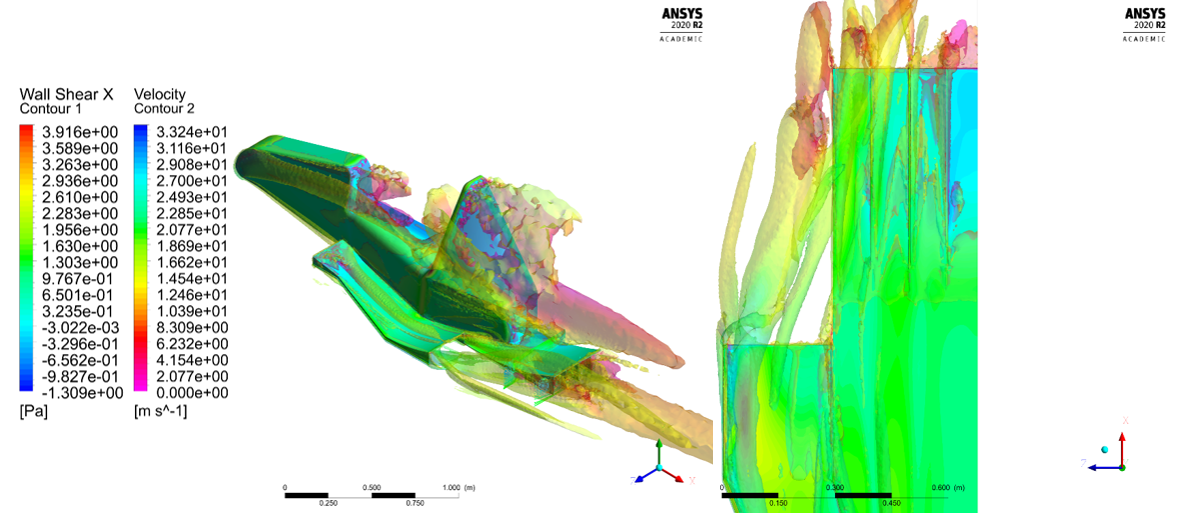
\includegraphics[width=1\textwidth]{Figures/UTP_FIGS/UTP_QCRIT_WSHEAR_COMPILE.png}}
    \caption{Undertray Prototype 2 with Bluff Body X Wall Shear and Velocity Contour of Q-Criterion of 0.005 .}
      \label{fig:3D_QCRIT_WSHEAR_UTP2}
\end{figure}

\noindent \textbf{Figure \ref{fig:3D_QCRIT_WSHEAR_UTP2}}  shows the X wall shear on the bluff body and vortices indicated by the Q-Criterion. Similar to the previous analysis, the negative X Wall-Shear indicated the separation region on the undertray. Similar to all previous analysis, flow attachment is a crucial facet in improving the overall performance. Vertices formed at the rear generated by the vortex generator play a crucial role in affecting the undertray's performance. A good undertray design is graded by its effectiveness to capture or trap the vortices, which creates a suction effect \cite{Bouferrouk2014OnVehicles}; hence, higher downforce and traction can be achieved. It can be seen from the figure \ref{fig:3D_QCRIT_WSHEAR_UTP2} above that the flow stays attached on the diffuser region where vortex formed, and the blue region on the middle of the diffuser are indicating flow separation where vortex formation is not prominent. UTP 2,5,6, and 7 have similar side-diffuser geometry; however, each undertray's diffuser geometries is distinct. UTP 5, 6, and 7 have a higher angle variable on the outermost; this allows a larger vortex generated, which generated a slight increase in downforce (see table \ref{UTB_RESULTS}).

\noindent Nonetheless, ineffective vortex generation, which causes shedding, induced early flow separation on the diffuser's boundary layer, causing a significant drag increase. It can be seen from \textbf{figure \ref{fig:UTP_BOTTOM_QCRIT_ALL_COMPARE} in Appendix D} that region of outermost diffuser angle of UTP 5, 6, and 7 shows lower x wall-shear value (indicated by the light blue region), suggesting that flow separation occurred at that region which generated unstably and shedding vortex, hence drag increase. Comparing undertray with similar lift value (e.g. UTP 2, 5, 6, and 7), it was suspected from figure \ref{fig:UTP_BOTTOM_QCRIT_ALL_COMPARE} and \ref{fig:UTP_ISO_QCRIT_ALL_COMPARE} that undertray with higher drag (UTP 5, 6, and 7) has unstructured vortices near the outlet that may indicate vortex instability, compared to UTP2 which has cleaner trailing vortex. Moreover, the curved side diffuser sculpts the inlet's flow sideways, which increases the acceleration and decreases the pressure. This condition generated a sizeable corner vortex and low-pressure region at the turning point, increased the trapped vortex's size, and increased the overall downforce.

\noindent However, the simulation used a clean bluff-body which allows clean air to enter the inlet region on both nose and side diffuser. This is not ideal in real-life case, as several parts, such as; suspensions, tyres, and front wing (future design), might disturb the incoming flow and affect the vortex generation at the rear. It can be concluded that downforce improvement and drag reduction is the matter of flow strategy and management for effective flow control to achieve a stable vortex using intelligent analysis and advanced undertray design; therefore, focusing on stable vortex generation shall be the priority for future work in the undertray design. Another limitation is all the simulations were done in a partial model. A paper by Senior \cite{Senior2001TheEffect} suggested the importance of symmetric flow in high-performance undertray, and the analyses in this paper assumed a symmetrical flow in the simulation. Hence, in a forthcoming paper, it is also important that the undertray simulation is done with whole geometry.
















